% Tradepilot: technical report
% Build: pdflatex technical_report.tex   (run twice for the table of contents)
% Uses only standard packages (TeX Live / MiKTeX / Overleaf).
\documentclass[11pt,a4paper]{article}

\usepackage[margin=2.4cm]{geometry}
\usepackage[T1]{fontenc}
\usepackage[utf8]{inputenc}
\usepackage{lmodern}
\usepackage{microtype}
\usepackage{amsmath,amssymb}
\usepackage{booktabs}
\usepackage{tabularx}
\usepackage{array}
\usepackage{enumitem}
\usepackage{xcolor}
\usepackage{tikz}
\usetikzlibrary{positioning,arrows.meta}
\usepackage[hidelinks]{hyperref}

\definecolor{accent}{HTML}{2457D6}
\newcommand{\code}[1]{\texttt{\small #1}}
\newcolumntype{L}{>{\raggedright\arraybackslash}X}
\setlist{itemsep=2pt,topsep=4pt}

\title{\textbf{Tradepilot}\\[4pt]
\large A deterministic crypto trading system for OKX demo trading:\\
design, research method, live validation and lessons}
\author{Project repository: \code{github.com/sa1ffffff/tradepilot}}
\date{23 October 2026}

\begin{document}
\maketitle

\begin{abstract}
\noindent Tradepilot is a pair of deterministic trading bots, one for spot and one for
USDT-margined perpetual swaps, that trade a user's OKX \emph{demo} (simulated) account from
a local PC, together with the research tooling used to choose what they trade. The system
deliberately keeps any language model out of the trading loop: signals come from indicator
rules, sizing and limits from a hard-coded risk layer, and strategies are admitted only after
an anchored walk-forward test on up to three years of history scored on data the parameters
never saw. This report describes the architecture, the cost model, the research method and its
results, a 46-hour live demo run and what it measured, and the changes made because of it.
The headline engineering result is that the backtest is a faithful model of the live bots:
all 10 spot entries and all 3 futures entries in the demo run matched their backtest
counterparts. The headline research result is that trading costs, not indicator choice,
decide whether a short-horizon strategy can be profitable: no spot strategy survived on
15-minute bars, while a set of 4-hour perpetual-swap strategies passed out of sample and is
now in a multi-week forward test. Nothing in this report is financial advice; all trading
described is with simulated funds.
\end{abstract}

\tableofcontents
\bigskip

%=====================================================================
\section{Goals and constraints}
%=====================================================================
The project began as a request to build a bot that ``trades on OKX and is profitable on one or
two days of recorded data''. Two constraints shaped everything that followed.

\begin{enumerate}
\item \textbf{One or two days cannot show profitability.} A strategy that trades a few times a
day produces a handful of trades in two days; their total P\&L is dominated by noise. Tuning
parameters until a short window looks profitable is curve-fitting. The phase-1 goal was
therefore restated as two checkable questions: (a) does a strategy show an edge on months of
data it was \emph{not} tuned on, and (b) does the live bot do exactly what the backtest says it
would over the same hours?
\item \textbf{The decision loop must be deterministic and auditable.} Large language models are
slow, non-deterministic and costly per call; markets punish all three. Claude's role is to build,
test and review the system and to analyse results, never to place a trade.
\end{enumerate}

\noindent Operational constraints: everything runs on the user's Windows PC; OKX demo trading
only (\code{DEMO=true}, live mode is refused); the API key has Read and Trade permission but never
Withdraw; secrets live only in an untracked \code{.env}.

%=====================================================================
\section{System architecture}
%=====================================================================
\begin{figure}[h]
\centering
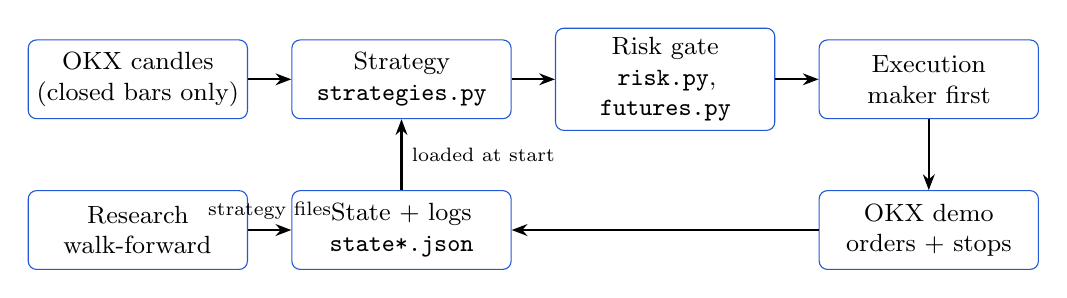
\begin{tikzpicture}[
  box/.style={draw=accent, rounded corners=3pt, align=center, minimum height=1.0cm,
              text width=2.55cm, font=\small},
  arr/.style={-{Stealth[length=2mm]}, thick}]
\node[box] (data) {OKX candles\\(closed bars only)};
\node[box, right=0.55cm of data] (strat) {Strategy\\\code{strategies.py}};
\node[box, right=0.55cm of strat] (risk) {Risk gate\\\code{risk.py}, \code{futures.py}};
\node[box, right=0.55cm of risk] (exec) {Execution\\maker first};
\node[box, below=0.9cm of exec] (okx) {OKX demo\\orders + stops};
\node[box, below=0.9cm of strat] (state) {State + logs\\\code{state*.json}};
\node[box, below=0.9cm of data] (research) {Research\\walk-forward};
\draw[arr] (data) -- (strat);
\draw[arr] (strat) -- (risk);
\draw[arr] (risk) -- (exec);
\draw[arr] (exec) -- (okx);
\draw[arr] (okx) -- (state);
\draw[arr] (research) -- node[above, font=\scriptsize]{strategy files} (state);
\draw[arr] (state) -- node[right, font=\scriptsize]{loaded at start} (strat);
\end{tikzpicture}
\caption{Data flow. Research writes JSON strategy files; the bots load them at start-up. The
same signal and simulation code serves research, backtests and the live bots.}
\end{figure}

\subsection{Components}
\begin{table}[h]
\centering\small
\begin{tabularx}{\textwidth}{@{}lL@{}}
\toprule
Module & Responsibility \\
\midrule
\code{bot/strategies.py} & Nine long-only strategies (EMA cross, trend pullback, Donchian
breakout, Bollinger reversion, Supertrend, and four cost-aware variants with ADX and
higher-timeframe trend filters and a chandelier exit), plus a mirrored short version for swaps.
Each maps closed candles to \code{entry}/\code{exit} columns. \\
\code{bot/indicators.py} & EMA, RMA-smoothed RSI and ATR, Bollinger bands, ADX, Supertrend,
chandelier level; computed as TradingView computes them, causally. \\
\code{bot/engine.py} & Bar-by-bar simulation for spot (\code{simulate}) and swaps
(\code{simulate\_ls}): fees, slippage, stops, take-profit, trailing stop, funding, liquidation. \\
\code{bot/costs.py} & Cost model shared by engine, risk gate and bots (Section~\ref{sec:costs}). \\
\code{bot/risk.py} & Position sizing, notional cap, daily loss limit, cost gate, signal
de-duplication, persistence. \\
\code{bot/futures.py} & Swap sizing, volatility-based leverage, trailing-stop rule. \\
\code{bot/runner.py}, \code{bot/futures\_runner.py} & The live loops (spot long/flat; swaps
long/short, up to one strategy per coin). \\
\code{bot/exchange.py}, \code{bot/futures\_exchange.py} & ccxt wrappers: maker-first orders,
fill aggregation, exchange-side stop orders. \\
\code{bot/lock.py} & Operating-system file lock so a second copy of a bot cannot start. \\
\code{research.py}, \code{timemachine.py} & Walk-forward research; Monte-Carlo replay of
out-of-sample trades. \\
\code{session\_report.py}, \code{futures\_session\_report.py}, \code{demo\_report.py} &
Live-versus-backtest reconciliation and run reports. \\
\code{dashboard.py} & Read-only local web dashboard (\code{127.0.0.1:8765}). \\
\code{check\_connection.py}, \code{check\_futures.py} & Read-only account checks (keys,
permissions, fees, sizes); never place orders. \\
\bottomrule
\end{tabularx}
\caption{Main modules. The test suite has 95 tests and runs offline against fake exchanges.}
\end{table}

\subsection{Design rules}
\begin{itemize}
\item \textbf{One code path.} \code{signals()} and the simulators are used by research, the
backtest, the reconciliation reports and (for signals) the live bots, so what is tested is what
trades.
\item \textbf{Closed bars only.} The still-forming candle is dropped by timestamp, never by
position.
\item \textbf{The bot owns only its own position.} OKX demo accounts start pre-funded with BTC;
the spot bot tracks its position in \code{state.json} and only ever sells what it bought.
\item \textbf{Crash-safe state.} State is written atomically after every change; the daily loss
counter survives restarts.
\item \textbf{One instance.} A per-state-file OS lock (released automatically on exit or crash)
makes a second copy exit. This was added after two spot bots were found running at once.
\end{itemize}

%=====================================================================
\section{Execution, risk and the cost model}\label{sec:costs}
%=====================================================================
\subsection{Orders}
With \code{EXECUTION=maker}, an order is first posted as a post-only limit at the best bid
(buy) or ask (sell), waits up to 20\,s, is re-priced up to three times, and any remainder goes
as a market order. Stop-loss exits always go straight to market. Each fill records its maker
share, so the real fill rate can be measured.

\subsection{Cost model}
Let $f_m$ and $f_t$ be the maker and taker fee rates, $s$ the market-order slippage and $r$ the
share of maker attempts that fill. The expected cost per side of a normal (non-stop) fill and of
a stop fill are
\begin{equation}
c_{\text{passive}} = r\,f_m + (1-r)\,(f_t + s), \qquad c_{\text{stop}} = f_t + s .
\end{equation}
OKX regular-tier spot fees are $f_m=0.08\%$, $f_t=0.10\%$; swap fees $0.02\%$ and $0.05\%$; $s$ is
taken as 2\,bps. Research initially assumed $r=0.70$; the demo run measured $r=0.54$ on spot
(Section~\ref{sec:demo}), which is now the default.

\paragraph{Cost gate.} An entry with stop distance $d$ at price $P$ is skipped when round-trip
costs would exceed a fraction $k$ (default 0.2) of the amount risked:
\begin{equation}
2\,c_{\text{passive}}\,P > k\,d .
\end{equation}
With a tight stop the fees alone can be a large share of every loss; this rule is what made 15-
minute spot strategies untradeable (Section~\ref{sec:spot-research}).

\subsection{Spot sizing}
With equity $E$, risk fraction $f$ (1\%), stop distance $d=a\cdot\mathrm{ATR}$ and cap
$N_{\max}$ (\$1{,}000 in the demo):
\begin{equation}
q = \min\!\left(\frac{E f}{d},\; \frac{E}{P(1+c_{\text{stop}})},\; \frac{N_{\max}}{P}\right),
\end{equation}
i.e.\ risk-based, but never more than cash (no hidden leverage in a spot account) and never above
the hard cap. A daily loss limit blocks new entries for the rest of the UTC day.

\subsection{Swap sizing and leverage}
Swaps size the same way with $f=2\%$, but leverage is derived from volatility so that the
liquidation price is at least $b=3$ times further away than the stop:
\begin{equation}
L = \min\!\left(L_{\max},\; \left\lfloor \frac{1}{b\,d/P + m} \right\rfloor\right),
\end{equation}
with maintenance margin $m=0.4\%$ and $L_{\max}=5$. Margin is isolated, and total margin across
all open positions is capped at 50\% of equity; a position that would exceed it is shrunk. A
strategy file may instead fix the position value (used only for a demo test slot).

\subsection{Stops on the exchange}
Every swap position has its stop resting on OKX as an algo order that closes the whole
position, so it protects the account even if the PC or bot stops. A missing stop is re-placed on
the next poll; if placement fails the position is closed at once; a position whose liquidation
price would sit inside the stop is closed.

\subsection{Trailing stop}
Once the best price since entry, $x$, is at least $R_0$ times the initial risk $d_0$ in profit,
the stop follows it at $\mu$ times the strategy's stop distance, and only tightens:
\begin{equation}
\text{stop}_t = \begin{cases}
\max\!\big(\text{stop}_{t-1},\; x - \mu\,a\,\mathrm{ATR}_t\big) & \text{long, if } x-P_0 \ge R_0 d_0\\
\text{stop}_{t-1} & \text{otherwise.}
\end{cases}
\end{equation}
Live, the new OKX stop is placed before the old one is cancelled. The same rule runs in the
swap simulator. Defaults are $R_0=2$, $\mu=2$ (Section~\ref{sec:trail}).

\subsection{Failure handling}
A signal is marked as handled before its order is sent, so a lost reply cannot cause a second
entry. If an entry errors, the next poll checks OKX: with no position and no resting order nothing
went through and the signal is retried; otherwise it is not repeated. Failed exits are retried
immediately (they are reduce-only). This closed a gap found in the demo run
(Section~\ref{sec:demo}).

%=====================================================================
\section{Research method}
%=====================================================================
\subsection{Anchored walk-forward}
History is split into five equal segments $S_0,\dots,S_4$. For fold $k=1..4$, parameters are
chosen on $S_0\ldots S_{k-1}$ and traded unchanged on $S_k$. Only $S_1\ldots S_4$ (80\% of the
history, never seen at selection time) is reported. Parameters are chosen by the $t$-statistic of
per-trade returns,
\begin{equation}
t = \frac{\bar r}{s_r}\sqrt{n}, \qquad n \ge 10,
\end{equation}
which rewards consistency over one lucky trade.

\subsection{Pass criterion}
A strategy-market pair is a \textsc{candidate} only with at least 30 out-of-sample trades, profit
factor $\ge 1.2$, positive return, and at least 3 of 4 folds profitable. An ``auto'' row repeats
the process choosing among \emph{all} strategies in each fold; it is the most honest estimate of
what the research process itself is worth, because it pays for the selection.

\subsection{Guarding against luck}
Dozens of strategy-market pairs are tested per run, so some pass by chance. A candidate is more
credible when it also works on other coins, survives taker-only costs, holds on a second data
source (Crypto.com prices), and keeps working in a forward demo run. The \emph{time machine}
re-draws a strategy's out-of-sample trades 10{,}000 times (and whole calendar months for the
portfolio, so coins that crash together still crash together) to show the range of outcomes to
expect over a given horizon.

%=====================================================================
\section{Research results}
%=====================================================================
\subsection{Spot: costs decide}\label{sec:spot-research}
On 12 months of BTC and ETH, no strategy passed on 15\,m, 1\,h or 4\,h. The decomposition in
Table~\ref{tab:costs} shows why: several strategies have a small edge before costs that 0.24\%
round-trip (taker fees plus slippage) erases. On 15\,m a 2-ATR stop sits under 1\% from entry, so
costs are about a quarter of every unit risked.

\begin{table}[h]
\centering\small
\begin{tabular}{@{}lrr@{}}
\toprule
Strategy (default parameters, 12 months) & With costs & Zero costs \\
\midrule
BTC 15m Bollinger reversion & $-38.1\%$ & $+10.8\%$ \\
ETH 1h EMA cross & $-14.6\%$ & $+19.0\%$ \\
BTC 1h trend pullback & $-1.4\%$ & $+11.9\%$ \\
\bottomrule
\end{tabular}
\caption{Effect of trading costs on otherwise-plausible spot strategies.}\label{tab:costs}
\end{table}

\noindent After adding maker-first execution, the cost gate, wider stops and four cost-aware
1\,h/4\,h variants, a 3-year run found two spot candidates: BTC 4h chandelier trend ($+23.2\%$,
PF 1.82) and ETH 1h EMA cross with ADX ($+20.9\%$, PF 1.31). Neither survives taker-only costs,
neither works on the other coin, and the ``auto'' rows lose on every spot market, so they are
treated as unproven. At the measured 54\% fill rate both still pass ($+22.9\%$ and $+24.1\%$).

\subsection{Perpetual swaps}
Swaps differ in two ways that matter: fees are about a quarter of spot fees, and the strategies
can go short. On 3 years of 4\,h and 1\,h data across nine coins, many strategy-market pairs pass, and the
results barely move between a 70\% and a 54\% maker fill rate. On one year of 15-minute data,
by contrast, only 1 of 18 swap pairs passed. Eight 4\,h strategies form the current lineup
(Table~\ref{tab:lineup}).

\begin{table}[h]
\centering\small
\begin{tabular}{@{}llrrc@{}}
\toprule
Coin & Strategy (4h) & OOS return & PF & Folds $+$ \\
\midrule
ADA & Supertrend, long+short & $+88\%$ & 2.04 & 4/4 \\
AVAX & Supertrend, long+short & $+40\%$ & 1.41 & 3/4 \\
BNB & Donchian breakout & $+31\%$ & 1.45 & 4/4 \\
DOGE & Supertrend & $+82\%$ & 2.10 & 3/4 \\
ETH & Trend pullback, long+short & $+13\%$ & 1.33 & 3/4 \\
LTC & Bollinger reversion & $+15\%$ & 1.42 & 3/4 \\
SOL & Donchian breakout & $+29\%$ & 1.52 & 3/4 \\
XRP & Donchian breakout & $+76\%$ & 1.49 & 4/4 \\
\bottomrule
\end{tabular}
\caption{Forward-test futures lineup: out-of-sample results over 3 years at the measured
costs, with the trailing stop. The ``auto'' rows pass on only 4--5 of 18 swap markets,
a reminder that some of these are likely luck.}\label{tab:lineup}
\end{table}

\subsection{Trailing stop calibration}\label{sec:trail}
A tight trail (start at 1R, trail at 1$\times$ the stop distance) cut the summed 3-year return of
the eight research strategies from 568\% to 391\%: trend strategies earn from a few long runs that
a tight trail exits early. A loose trail (2R, 2$\times$) left it at 567\% while lowering the worst
drawdown on some coins (ETH 1h: $17.4\% \to 15.1\%$). The loose setting is the default; the tight
one was used only on a fast test slot, where it improved a 30-day result from $-41\%$ to $-32\%$.

\subsection{Can a ``solid'' signal be recognised at entry?}\label{sec:solid}
After one 5-minute test trade made about 10R, the question was whether such signals could be
sized up. Over 712 trades in 90 days that strategy averaged $-0.64$R with a 26\% win rate; seven
entry traits (ADX above 25 or 35, agreement with 16-hour and 2-day trends, volatility, and
combinations) produced no subgroup with positive expectancy. Only 2 of the 712 trades made about
10R. The outlier was luck, kept by the trailing stop; it was not predictable at entry.

%=====================================================================
\section{Live demo run (20--22 October 2026)}\label{sec:demo}
%=====================================================================
Both bots ran for 46 hours against the OKX demo account. Spot traded a deliberately fast
5-minute EMA test strategy (to exercise the plumbing); futures traded the research lineup plus a
5-minute BTC test slot.

\begin{table}[h]
\centering\small
\begin{tabular}{@{}lrrr@{}}
\toprule
Bot & Trades & Won & Net P\&L (USDT) \\
\midrule
Spot (BTC 5m test) & 10 & 1 & $-29.02$ \\
Futures (BTC 5m test slot) & 3 & 1 & $+146.80$ \\
\midrule
Total & 13 & 2 & $+117.78$ \\
\bottomrule
\end{tabular}
\caption{Demo run results (simulated funds, after fees; futures figures from OKX's records,
including funding).}
\end{table}

\paragraph{Fidelity.} Replaying the same hours on OKX's demo candles, \textbf{10 of 10} spot
entries and \textbf{3 of 3} futures entries matched their backtest trades, with entry prices
within a few basis points. Exits differ slightly where live stops trigger between bars or a
setting changed mid-run. This is the run's most important result: research is a faithful model
of the bots, so it, not a short live window, is the evidence on profitability.

\paragraph{Measured costs.} Maker fills: 54\% of spot entries and non-stop exits (8 of 15),
versus 70\% assumed; 6 of 6 on futures. Entry price versus signal close: $-2.3$\,bps on average
(range $-12.5$ to $+4.1$). Five of thirteen exits were stops.

\paragraph{Reliability.} The demo service returned 17 spot errors and 64 futures network
warnings in 46 hours (timeouts, ``system busy'' 50013, ``service unavailable'' 50001). Both bots
recovered from every one, but the futures reconciliation found that one ADA entry signal had been
lost to a 50001 error during the order; the retry logic in Section~\ref{sec:costs} fixes it.

\paragraph{The largest trade.} A BTC short opened at 84{,}486 and was closed by the trailing stop
at 81{,}330 for $+158.26$ USDT, about 10.5 times its risk. Section~\ref{sec:solid} shows why this was not a
repeatable signal.

%=====================================================================
\section{Defects found and fixed}
%=====================================================================
\begin{table}[h]
\centering\small
\begin{tabularx}{\textwidth}{@{}lL@{}}
\toprule
Defect & Fix \\
\midrule
Spot bot inferred its position from the wallet, so it would sell the demo account's pre-funded
BTC & Bot tracks its own position in \code{state.json} \\
Daily loss limit never updated live & Realised P\&L from actual fills, persisted \\
Risk was sized against a stop nothing enforced & Software stop (spot), exchange stop (swaps) \\
Spot sizing could exceed cash (implicit leverage) & Size capped at equity \\
Backtest omitted entry fees & Fees on both sides in the engine \\
\code{--limit 1000} silently returned 300 candles & Paged candle download \\
Logging raised on empty field dicts & Formatter fixed \\
\code{www.okx.com} unreachable on the user's network & Configurable \code{OKX\_HOSTNAME} \\
Two copies of a bot could run at once & OS file lock per state file \\
An OKX error mid-entry lost the signal & Retry when OKX shows nothing went through \\
\bottomrule
\end{tabularx}
\caption{Main defects, in the order found.}
\end{table}

%=====================================================================
\section{Monitoring and operations}
%=====================================================================
\begin{itemize}
\item \textbf{Dashboard:} \code{start\_dashboard.bat} serves a read-only page with bot status
(from the lock files), open positions at live demo prices, P\&L and recent trades.
\item \textbf{Health check:} a scheduled read-only task every 2 hours confirms exactly one copy of
each bot, scans both logs, and appends an OK/ATTENTION note to \code{logs/health.md}.
\item \textbf{Reports:} \code{demo\_report.py} (trades, P\&L, costs, errors, and
\code{measured\_costs.json} for the next research round); \code{session\_report.py} and
\code{futures\_session\_report.py} (trade-by-trade reconciliation, explaining missed signals by
downtime or deliberate skips).
\end{itemize}

%=====================================================================
\section{Forward test (from 22 October 2026)}
%=====================================================================
The forward test runs the Table~\ref{tab:lineup} lineup (2\% risk each, trailing stop from 2R,
50\% margin cap) and the spot BTC 4h chandelier strategy (up to \$1{,}000 per position) for at
least six weeks. The time machine gives the yardstick for two months of the futures portfolio:

\begin{table}[h]
\centering\small
\begin{tabular}{@{}lr@{}}
\toprule
Expected trades & $\approx 38$ \\
Typical result & $+16.6\%$ \\
Bad 1-in-20 result & $-18.5\%$ \\
Probability of being down & 24\% \\
Worst drawdown, typical / 1-in-20 & 14\% / 24\% \\
Losing streak, 1-in-20 & 13 trades \\
\bottomrule
\end{tabular}
\caption{Two-month outcome range for the futures lineup (10{,}000 replays of out-of-sample trades).}
\end{table}

\noindent The test stops for investigation if a live trade has no backtest counterpart (or vice
versa), a position is ever without its exchange stop, drawdown exceeds 25\%, a losing streak
exceeds 13, maker fills fall well below 54\%, or a bot repeatedly stops by itself. At the end, the
measured costs feed the next research round and a lessons file records what changed.

%=====================================================================
\section{Limitations}
%=====================================================================
\begin{itemize}
\item \textbf{Demo is not live.} OKX demo prints its own candles (same trend, different wicks),
and demo liquidity and fills are not real-market liquidity.
\item \textbf{Multiple testing.} Many pairs are tested; some candidates will be luck. The weak
``auto'' results and the single-coin nature of the spot candidates are the warning signs.
\item \textbf{Small samples.} 13 live trades and 6 futures maker fills measure plumbing and costs,
not edge.
\item \textbf{Regime dependence.} Three years of history contain a limited number of market
regimes; trend strategies depend on trends continuing to occur.
\item \textbf{Spot retry gap.} The spot bot does not yet retry an entry lost to an exchange error;
it trades about twice a month, and the reconciliation report would show such a miss.
\item \textbf{No real money.} The system refuses live mode in this phase; moving to real funds
would need, at minimum, the forward test passing, a small-size live phase, and a review of every
safety mechanism against real-market behaviour.
\end{itemize}

%=====================================================================
\section{Conclusion}
%=====================================================================
The project delivered a working, tested, deterministic trading stack on OKX demo with a research
process that reports only out-of-sample results, a live-versus-backtest reconciliation that
showed the backtest to be faithful, and a cost model calibrated from real fills. The research
itself is sobering in the useful way: on short timeframes costs dominate, apparent edges are easy
to find and hard to keep, and a single large winner says little. The 4-hour swap strategies are
the most credible candidates so far; the forward test will show whether they behave as their
out-of-sample record predicts.

\vfill
\noindent\rule{\linewidth}{0.4pt}\\
\footnotesize All trading described used simulated funds on OKX demo trading. This report is an
engineering document, not financial or investment advice.

\end{document}
